% Created 2012-09-12 Wed 17:01
\documentclass[11pt,serif]{beamer}

\usepackage[utf8]{inputenc}
\usepackage[T1]{fontenc}
\usepackage{fixltx2e}
\usepackage{graphicx}
\usepackage{longtable}
\usepackage{float}
\usepackage{wrapfig}
\usepackage{soul}
\usepackage{textcomp}
\usepackage{marvosym}
\usepackage{wasysym}
\usepackage{latexsym}
\usepackage{amssymb}
\usepackage{hyperref}
\tolerance=1000
\usepackage{fourier}
\providecommand{\alert}[1]{\textbf{#1}}

\title{Quiver practicum: building a high-quality consensus sequence from PacBio data}
\author{David Alexander, Patrick Marks}
\date{\today}
\hypersetup{
  pdfkeywords={},
  pdfsubject={},
  pdfcreator={Emacs Org-mode version 7.8.11}}

\begin{document}

\maketitle


\section{Intro}
\label{sec-1}
\begin{frame}[fragile]\frametitle{What is Quiver?}
\label{sec-1-1}

\begin{itemize}
\item A multiple-read consensus calling algorithm for PacBio reads
\item Takes multiple reads of a given DNA template, outputs best guess
     of template's identity
\item QV-aware hidden Markov model to model our sequencing errors; a greedy
     algorithm to find the maximum likelihood template.
\item \textbf{Can achieve accuracy >Q50 (i.e. >99.999\%) using pure      PacBio raw reads.}
\end{itemize}
\end{frame}
\begin{frame}[fragile]\frametitle{What Quiver isn't}
\label{sec-1-2}

\begin{itemize}
\item Quiver is NOT an ``error-correction'' algorithm
\item Quiver is NOT YET a 100\% polished piece of software
\begin{itemize}
\item Has worked well in practice \ldots{} but bugs may remain
\item Verification and testing process just beginning now
\end{itemize}
\end{itemize}
\end{frame}
\begin{frame}[fragile]\frametitle{Quiver workflow}
\label{sec-1-3}

\begin{itemize}
\item Quiver takes a pile of PacBio reads (with QV information) that are
    from the same underlying DNA template, and infers the template identity.
\item Needs to be fed a \verb~cmp.h5~ file (an alignment to a rough assembly,
    or an accurate reference).
\item \verb~cmp.h5~ must have all QV data tracks: must be generated via
    \verb~ResequencingQVs~ protocol in SMRTPortal.
\end{itemize}
\end{frame}
\begin{frame}[fragile]\frametitle{Quiver workflow diagram}
\label{sec-1-4}

   \begin{figure}
   \centering
     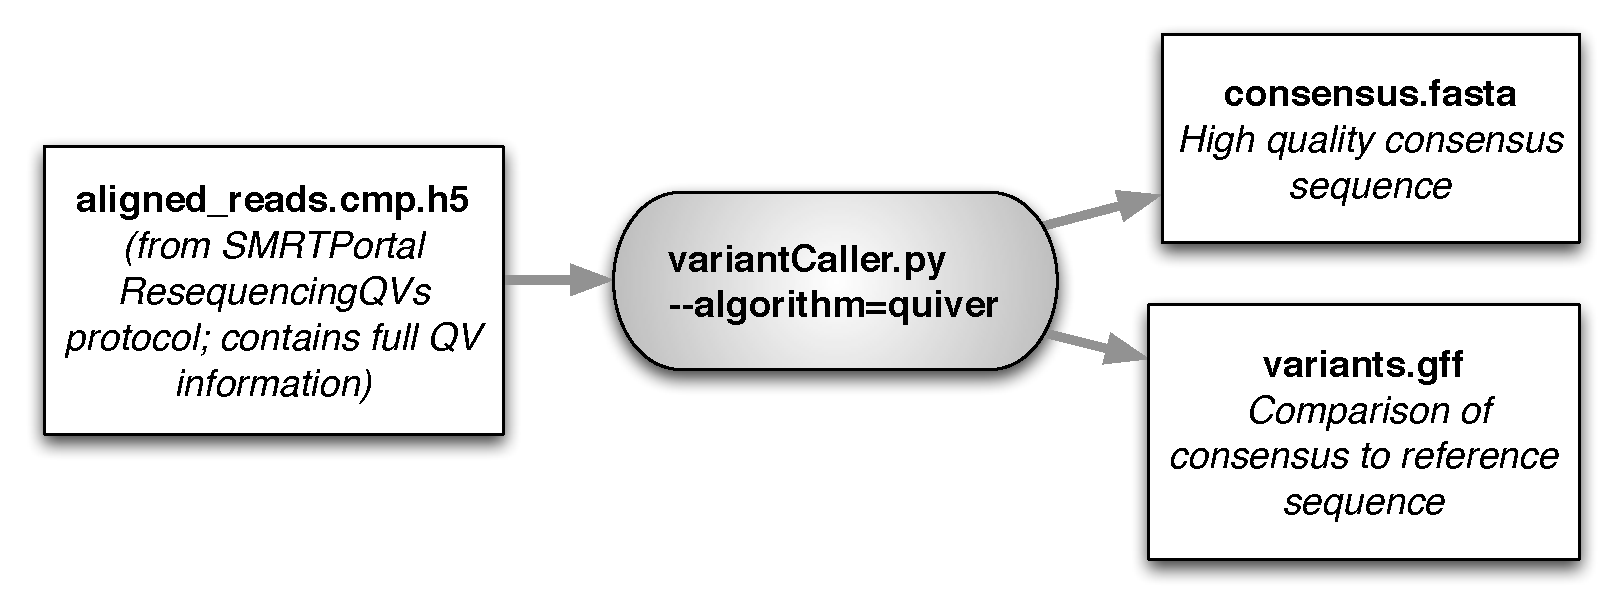
\includegraphics[width=4.5in]{img/quiver-workflow}
   \end{figure}
\end{frame}
\begin{frame}[fragile]\frametitle{Where does Quiver live?}
\label{sec-1-5}

\begin{itemize}
\item Driver program (\verb~variantCaller.py~) for Quiver is in
     \verb~GenomicConsensus~ (Python)
\begin{itemize}
\item requires the \verb~pbcore~ library for data file access
\item requires the \verb~ConsensusCore~ C++ library for core computational
       bits
\end{itemize}
\item Will be available in 1.4 SMRTportal, but for now requires custom
     installation of these packages and command line work.
\end{itemize}
\end{frame}
\begin{frame}[fragile]\frametitle{Let's install Quiver}
\label{sec-1-6}

   (Read \href{https://github.com/PacificBiosciences/GenomicConsensus/blob/master/doc/HowToQuiver.rst}{HowToQuiver document}
   for details and system requirements; this is just the gist of it!) \newline

   Install (root privileges not required):
   \begin{verbatim}
     $ curl -L git.io/JR7TnQ | bash
   \end{verbatim}

   Activate virtualenv via
   \begin{verbatim}
     $ source ~/VE-QUIVER/bin/activate
   \end{verbatim}
\end{frame}
\section{Resequencing consensus}
\label{sec-2}
\begin{frame}[fragile]\frametitle{Example: Resequencing consensus on an Lambda job}
\label{sec-2-1}

   Let's call resequencing-based consensus on a simple Lambda job!
   JobId 49002.
\begin{itemize}
\item 1 chip, 2 45'' movies; 2Kb insert size.  Mean coverage > 2800.
\item I've already run it through the \emph{ResequencingQVs} protocol
\end{itemize}

\begin{scriptsize}
\begin{verbatim}
$ export PB=/mnt/secondary/Smrtanalysis/
$ variantCaller.py -j2 --algorithm=quiver                                 \
   $PB/userdata/jobs/049/049002/data/aligned_reads.cmp.h5                 \
   -r $PB/opt/smrtanalysis/common/references/lambda/sequence/lambda.fasta \
   -o consensus.fasta -o variants.gff
\end{verbatim}
\end{scriptsize}

This command uses 100x coverage (subsamples) by default.
\end{frame}
\begin{frame}[fragile]\frametitle{Examine the output}
\label{sec-2-2}

\begin{itemize}
\item \verb~variants.gff~ contains \textbf{zero} variant entries!
\item The sequence in \verb~consensus.fasta~ is perfectly concordant with the
    lambda reference.
\end{itemize}

  We have effectively assembled a perfectly accurate lambda genome
  from a fraction of a single PacBio chip, only using the true
  reference to segregate reads together --- consensus is \textbf{de-novo}.
\end{frame}
\begin{frame}[fragile]\frametitle{Sidebar: comparing genomic sequences}
\label{sec-2-3}

I recommend using MUMmer 3.0 for comparing two FASTA files purpose. \newline

MUMmer includes a tool called \verb~dnadiff~

\begin{scriptsize}
\begin{verbatim}
$ dnadiff \
  $PB/opt/smrtanalysis/common/references/lambda/sequence/lambda.fasta \
  consensus.fasta
\end{verbatim}
\end{scriptsize}

Examine:
\begin{itemize}
\item \verb~out.report~ for a summary of differences
\item \verb~out.snps~ for SNPs;
\item \verb~gnuplot out.fg~ for a zoomable dot-plot.
\end{itemize}
\end{frame}
\begin{frame}[fragile]\frametitle{How was the reference used?}
\label{sec-2-4}

\begin{itemize}
\item Quiver only uses the alignment to the reference in order to group
  reads together.
\item Quiver's consensus calls are completely independent of
  the reference---only use the reads (\emph{Variant} calls still require
  reference for comparison.)
\end{itemize}
\end{frame}
\begin{frame}[fragile]\frametitle{Quiver's accuracy potential}
\label{sec-2-5}

   Indeed, we have found that Quiver can achieve accuracy >Q50 in
   real-world applications, even for true de-novo assemblies.  Recent
   examples:
\begin{itemize}
\item \emph{Meiothermus ruber}: Q37.5 before Quiver; Q50.6 after Quiver
     (including true variants)
\item \emph{Pedobacter heparinus}: QV51.5 after Quiver
\end{itemize}
\end{frame}
\section{Assembly consensus}
\label{sec-3}
\begin{frame}[fragile]\frametitle{Using Quiver for polishing an assembly}
\label{sec-3-1}

   Same basic workflow as for resequencing before, only modifications are:
\begin{itemize}
\item User needs to upload rough assembly FASTA to SMRTPortal as a
       new reference;
\item Then user needs to align against rough assembly in ResequencingQVs protocol
\item Then, same as before!
\item Output FASTA has same contigs as rough assembly, but accuracy
       will be higher.
\end{itemize}
\end{frame}
\begin{frame}[fragile]\frametitle{This workflow is a hack}
\label{sec-3-2}

   We will be making streamlining this workflow for the next SW release!
\end{frame}
\begin{frame}[fragile]\frametitle{Step 1: Building the assembly}
\label{sec-3-3}

Step 1: build the best rough assembly (high N50, low \# contigs) you
can using PacBio or 3rd Party workflows. \newline

Example: use \emph{RS\_Assembly} workflow with genome size set to good
estimate.

\begin{itemize}
\item Important to manually inspect output.  Bogus contigs?
\item \verb~mummerplot~ can be used to compare assembly to a reference.  Here
  are 3-contig and 1-contig lambda assemblies vs refererence.

   \begin{figure}
   \centering
     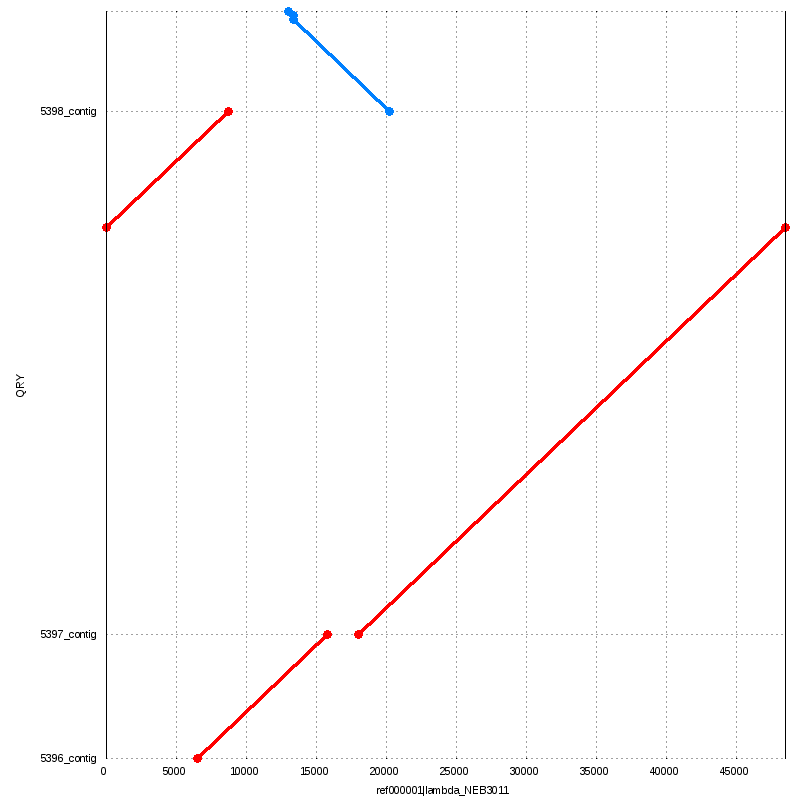
\includegraphics[width=1.5in]{img/lambda-3contig-assembly.png}
     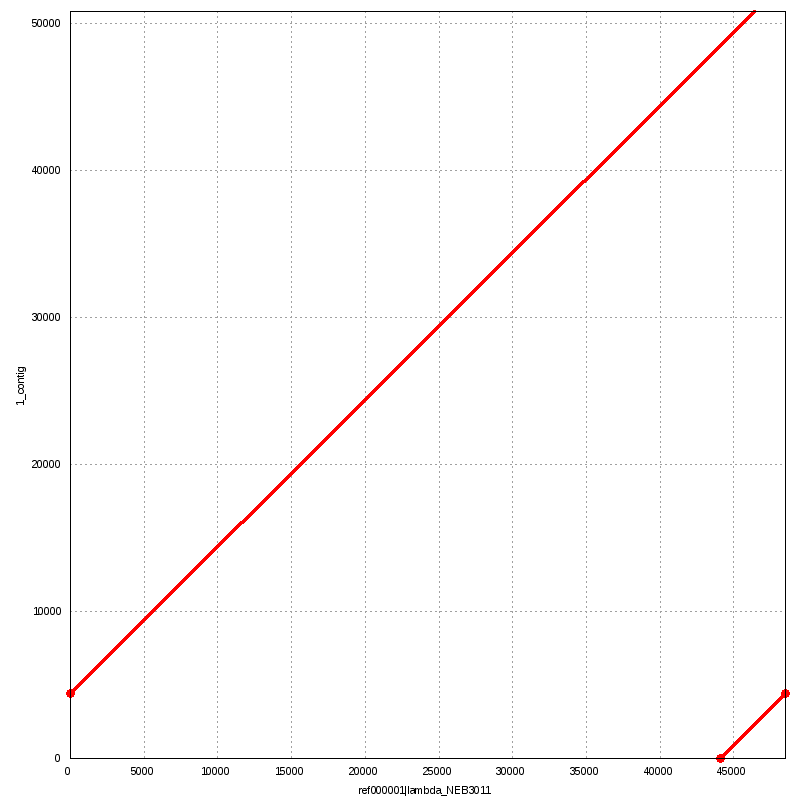
\includegraphics[width=1.5in]{img/lambda-1contig-assembly.png}
   \end{figure}
\end{itemize}
\end{frame}
\begin{frame}[fragile]\frametitle{Step 2: Uploading the assembly as a new reference}
\label{sec-3-4}

Upload the (curated) rough assembly FASTA file as a new reference to SMRTPortal
\end{frame}
\begin{frame}[fragile]\frametitle{Step 3: Align to the rough assembly using \emph{ResequencingQVs}}
\label{sec-3-5}

Select \emph{ResequencingQVs}, and select the reference you have just uploaded \newline

Example: My job was run and placed in Job 049061
\end{frame}
\begin{frame}[fragile]\frametitle{Step 4: Invoke Quiver}
\label{sec-3-6}

\begin{scriptsize}
\begin{verbatim}
$ export PB=/mnt/secondary/Smrtanalysis/
$ variantCaller.py -j2 --algorithm=quiver                                 \
   $PB/userdata/jobs/049/049061/data/aligned_reads.cmp.h5                 \
   -r assembled-1contig.fasta                                             \
   -o consensus.fasta -o variants.gff
\end{verbatim}
\end{scriptsize}
\end{frame}
\begin{frame}[fragile]\frametitle{Step 5: Examine accuracy}
\label{sec-3-7}

   You can use \verb~dnadiff~ as before to give rough accuracy metrics, or
   you can use \verb~blasr -m 0~ to give text visualizations of alignments.

   \newline
   Ex:
   \begin{scriptsize}
   \begin{verbatim}
   $ blasr lambda.fasta consensus.fasta -sa lambda.fasta.sa \
       -m 0 -out quiver-blasr.out
   \end{verbatim}
   \end{scriptsize}

   \newline
   Output snippet:

   \begin{scriptsize}
   \begin{verbatim}
   ...
   50  GGCGTTTCCGTTCTTCTTCGTCATAACTTAATGTTTTTATTTAAAATACC
    .  ||||||||||||||||||||||||||||||||||||||||||||||||||
 4461  GGCGTTTCCGTTCTTCTTCGTCATAACTTAATGTTTTTATTTAAAATACC
   ...
   \end{verbatim}
   \end{scriptsize}

   \textbf{Quiver accuracy should be substantially better than rough     assembly!!}
\end{frame}
\section{Quiver pitfalls and troubleshooting}
\label{sec-4}
\begin{frame}[fragile]\frametitle{Effective coverage dips and \verb~MapQV~}
\label{sec-4-1}

\begin{itemize}
\item As you would expect Quiver accuracy, scales with coverage.
\item \verb~variantCaller.py~ filters out reads with low \verb~MapQV~, so long
     repeats in the genome can end up inducing effective coverage
     deserts, and errors can pile up there.
\item We will be adding diagnostic plots to show these\ldots{}
\end{itemize}
\end{frame}
\begin{frame}[fragile]\frametitle{Mixed samples}
\label{sec-4-2}

Quiver expects to be running on an unmixed, homogeneous sample
\begin{itemize}
\item Do not feed diploid data to Quiver! (yet)
\item If there is suspicion of a mixed sample, examine Quiver output
    carefully.
\end{itemize}
\end{frame}
\begin{frame}[fragile]\frametitle{Error profile}
\label{sec-4-3}

Quiver still makes occasional errors.  By and large, these will be
indels in homopolymer regions, but they should be very rare, given
adequate coverage.  We have found great results with coverage >50x.

   \begin{scriptsize}
   \begin{verbatim}
   ...
  2200  AACTCTCACTCC-AAAAAAAAAAAAAAAAAAAAAAAAAGTCTAAATGCTT
     .  |||||||||||| |||||||||||||||||||||||||||||||||||||
 32848  AACTCTCACTCCAAAAAAAAAAAAAAAAAAAAAAAAAAGTCTAAATGCTT
   ...
   \end{verbatim}
   \end{scriptsize}
\end{frame}
\section{Conclusions}
\label{sec-5}
\begin{frame}[fragile]\frametitle{Conclusions}
\label{sec-5-1}

\begin{itemize}
\item Quiver is used to improve accuracy of pure-PacBio consensus
     results: >Q50 attainable.
\item Requires cmpH5 produced via \emph{ResequencingQVs} worfklow
\item \textbf{De-novo} consensus; reference not used to inform consensus
     calls.
\item Quiver will be pre-packaged in SMRTPortal in the next major
     software release.
\end{itemize}
\end{frame}

\end{document}
